% Компилировать с помощью: pdflatex, xelatex или lualatex
\documentclass[8pt, aspectratio=169]{beamer}
\usepackage[utf8]{inputenc}
\usepackage[russian]{babel}
\usepackage{amsmath, amssymb, amsfonts}
\usepackage{graphicx}
\usepackage{hyperref}
\usepackage{xcolor}
\usepackage{wrapfig}
\usepackage{float}
\usepackage{gensymb}
\usepackage{textcomp}
\usepackage{multirow}

% Настройка цвета формул
\definecolor{mathcolor}{RGB}{139,69,19} % brown
\everymath{\color{mathcolor}}
\everydisplay{\color{mathcolor}}
\linespread{1.2}

% Настройка темы Beamer
\usetheme{Madrid}
\usecolortheme{default}

% Убираем навигационные символы
\setbeamertemplate{navigation symbols}{}

% Заголовок
\title{Комплексные числа}
\author{}
\date{}

\begin{document}

% Титульный слайд
\begin{frame}
\titlepage
\end{frame}

% Слайд 1: Мотивация
\begin{frame}{Мотивация}
\textbf{Почему стоило рассказать о комплексных числах в школьном спринте?}

\begin{itemize}
    \item интегрируют в себе идеи из функций, тригонометрии, экспоненты, векторов, а это значит возможность посмотреть взаимосвязь этих понятий.
    \item применяются при решении уравнений, в теории чисел, комбинаторике, вычислении логарифмов из отрицательных чисел, тригонометрических уравнений вида $\cos(x) = c, \; c > 1$
    \item личный вызов, по мере подготовки презентации вскрываются пробелы в понимании комплексных чисел и тех школьных понятий, которые с ними связаны.
\end{itemize}
\end{frame}

% Слайд 2: Натуральные числа
\begin{frame}{Натуральные числа}
\textbf{Откуда взялись комплексные числа?}

\vspace{0.3cm}

$\mathbb{N}$ - \textbf{натуральные числа}:
\begin{flushleft}
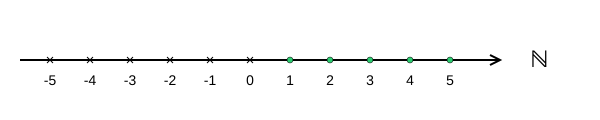
\includegraphics[width=0.5\textwidth]{./images/numbers/N_numbers.png}
\end{flushleft}

\textbf{Операции:}
\begin{itemize}
    \item[\checkmark] $a + b = c$, где $a, b, c \in \mathbb{N}$
    \item[x] $a - b = c$, где $a, b, c \in \mathbb{N}$, но только при $a > b$
    \item[\checkmark] $a \cdot b = c$, где $a, b, c \in \mathbb{N}$
    \item[x] $a/b = c$, где $a, b \in \mathbb{N} \iff a \mathbin{\vdots} b$
    \item[x] $\sqrt{a} = c$, где $a, c \in \mathbb{N} \iff a = b^2, \; b \in \mathbb{N}$
\end{itemize}
\end{frame}

% Слайд 3: Целые числа
\begin{frame}{Целые числа}
$\mathbb{Z}$ - \textbf{целые числа}:
\begin{flushleft}
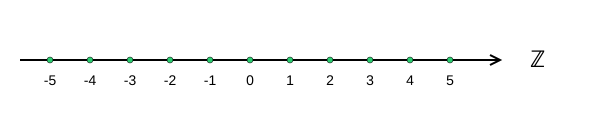
\includegraphics[width=0.5\textwidth]{./images/numbers/Z_numbers.png}
\end{flushleft}

\textbf{Операции:}
\begin{itemize}
    \item[\checkmark] $a + b = c$, где $a, b, c \in \mathbb{Z}$
    \item[\checkmark] $a - b = c$, где $a, b, c \in \mathbb{Z}$
    \item[\checkmark] $a \cdot b = c$, где $a, b, c \in \mathbb{Z}$
    \item[x] $a / b = c$, где $a, b, c \in \mathbb{Z} \iff a \mathbin{\vdots} b$
    \item[x] $\sqrt{a} = c$, где $a, c \in \mathbb{Z} \iff a = b^2, b \in \mathbb{Z}$
\end{itemize}

\textbf{Итог:} $\mathbb{N} \subset \mathbb{Z}$
\end{frame}

% Слайд 4: Рациональные числа
\begin{frame}{Рациональные числа}
$\mathbb{Q}$ - \textbf{рациональные числа}
\begin{flushleft}
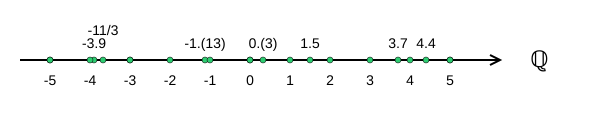
\includegraphics[width=0.5\textwidth]{./images/numbers/Q_numbers.png}
\end{flushleft}

\textbf{Операции:}
\begin{itemize}
    \item[\checkmark] $a + b = c$, где $a, b, c \in \mathbb{Q}$
    \item[\checkmark] $a - b = c$, где $a, b, c \in \mathbb{Q}$
    \item[\checkmark] $a \cdot b = c$, где $a, b, c \in \mathbb{Q}$
    \item[\checkmark] $a / b = c$, где $a, b, c \in \mathbb{Q}$
    \item[x] $\sqrt{a} = c$, где $a, c \in \mathbb{Q} \iff a = b^2, b \in \mathbb{Q}$
\end{itemize}

\textbf{Итог:} $\mathbb{N} \subset \mathbb{Z} \subset \mathbb{Q}$
\end{frame}

% Слайд 5: Иррациональные числа
\begin{frame}{Иррациональные числа}
$\mathbb{I}$ - \textbf{иррациональные числа}:
\begin{flushleft}
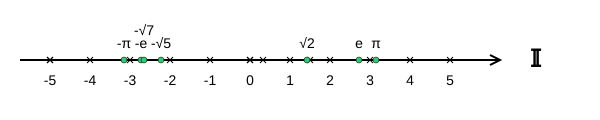
\includegraphics[width=0.5\textwidth]{./images/numbers/I_numbers.png}
\end{flushleft}

\begin{itemize}
    \item $\pi, e, \sqrt{2}, -\sqrt{3}$
\end{itemize}

Появляются при попытке, например, найти длину гипотенузы треугольника с катетами длиной $1$:

\begin{flushleft}
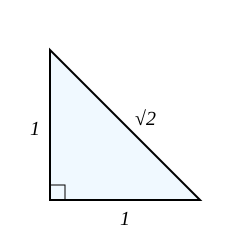
\includegraphics[width=0.3\textwidth]{./images/triangle.png}
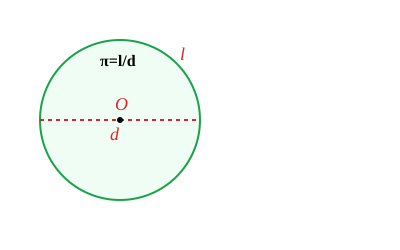
\includegraphics[width=0.4\textwidth]{./images/circle.png}
\end{flushleft}
\end{frame}

\begin{frame}{Иррациональные числа}
\textbf{Операции:}
\begin{itemize}
    \item[x] $a + b = c$, где $a, b \in \mathbb{I}$, $c \in \mathbb{I}$ или $c \in \mathbb{Q}$
    \item[x] $a - b = c$, где $a, b \in \mathbb{I}$, $c \in \mathbb{I}$ или $c \in \mathbb{Q}$
    \item[x] $a \cdot b = c$, где $a, b \in \mathbb{I}$, $c \in \mathbb{I}$ или $c \in \mathbb{Q}$
    \item[x] $a / b = c$, где $a, b \in \mathbb{I}$, $c \in \mathbb{I}$ или $c \in \mathbb{Q}$
    \item[\checkmark] $\sqrt{a} = c$, где $a, c \in \mathbb{I}$
\end{itemize}
\end{frame}

% Слайд 6: Действительные числа
\begin{frame}{Действительные числа}
$\mathbb{R}$ - \textbf{действительные числа}:

\begin{flushleft}
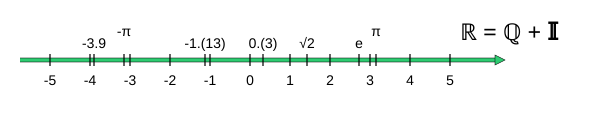
\includegraphics[width=0.5\textwidth]{./images/numbers/R_numbers.png}
\end{flushleft}

\begin{itemize}
    \item[\checkmark] $a + b = c$, где $a, b, c \in \mathbb{R}$
    \item[\checkmark] $a - b = c$, где $a, b, c \in \mathbb{R}$
    \item[\checkmark] $a \cdot b = c$, где $a, b, c \in \mathbb{R}$
    \item[\checkmark] $a / b = c$, где $a, b, c \in \mathbb{R}$
    \item[x] $\sqrt{a} = c$, где $a, c \in \mathbb{R} \iff a \ge 0$
\end{itemize}

\textbf{Итог:} $\mathbb{N} \subset \mathbb{Z} \subset \mathbb{Q} \subset \mathbb{R}$ \\
$\mathbb{R} = \mathbb{Q} + \mathbb{I}$ \\
$\mathbb{R}$ содержит все точки на прямой, \textbf{нет дыр} (пробелов)
\end{frame}

% Слайд 7: Комплексные числа - начало
\begin{frame}{Предыстория комплексных чисел}

\textbf{Комплексные числа} $\mathbb{C}$ возникли при необходимости обойти ограничение, связанное с \textbf{вычислением отрицательных корней}.

Рафаэль Бомбелли в своей работе «Алгебра» (1572г.) разобрал уравнение, которое поставило в тупик его современников. Это уравнение:

$$
x^3=15x+4
$$

Если использовать формулу Кордано, то получим:
$$
x = \sqrt[3]{2+\sqrt{-121}} + \sqrt[3]{2-\sqrt{-121}}
$$
т.е. \textbf{решений нет}

Но если взять $x=4$, то $4^3=15\cdot4+4=64$, то решение оказывается есть.

Если временно согласиться с тем, что корень из отрицательного числа существует, то при дальнейших вычислениях мы придём к действительным корням.
\end{frame}

% Слайд 8: Догадка Бомбелли
\begin{frame}{Предыстория комплексных чисел}
Он догадался, что:
$$
\sqrt[3]{2+\sqrt{-121}} = \sqrt[3]{2+11\sqrt{-1}} = a + \sqrt{-b}
$$
$$
\sqrt[3]{2-\sqrt{-121}} = \sqrt[3]{2-11\sqrt{-1}} = a - \sqrt{-b}
$$

И методом подбора он определил, что $a=2, \; b=1$

И действительно:

$$
(2+\sqrt{-1})^3 = 2^3 + 3 \cdot 2^2 \cdot \sqrt{-1} + 3 \cdot 2 \cdot (\sqrt{-1})^2 + (\sqrt{-1})^3 = 2 + 11\sqrt{-1}
$$
$$
(2-\sqrt{-1})^3 = 2^3 - 3 \cdot 2^2 \cdot \sqrt{-1} + 3 \cdot 2 \cdot (\sqrt{-1})^2 - (\sqrt{-1})^3 = 2 - 11\sqrt{-1}
$$

В итоге получаем:
$$
x = \sqrt[3]{2+\sqrt{-121}} + \sqrt[3]{2-\sqrt{-121}}
$$
$$
x = 2 + 11\sqrt{-1} + 2 - 11\sqrt{-1} = 4
$$
\end{frame}


% Слайд 10: Куда поместить C?
\begin{frame}{Комплексные числа}
Где же должны располагаться комплексные числа $\mathbb{C}$, если нет дыр на действительной прямой $\mathbb{R}$.
Ответ, за пределы прямой $\mathbb{R}$, т.е. на плоскости.

Но прежде чем переходить к комплексной плоскости, разберем некоторые моменты.

К компл\textbf{е}ксным числам необходимо подходить к\textbf{о}мплексно.
\end{frame}

% Слайд 11: Понимание числа π
\begin{frame}{Понимание числа $\pi$}

\begin{wrapfigure}{l}{0.5\textwidth}
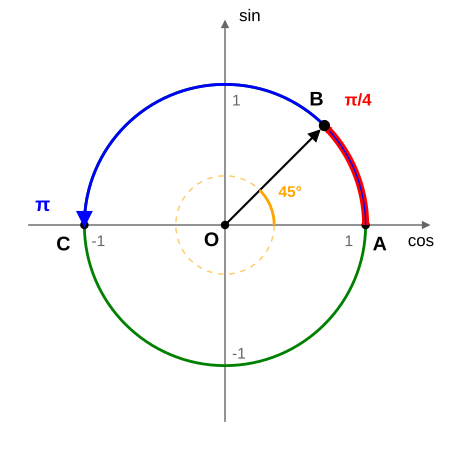
\includegraphics[width=0.45\textwidth]{./images/trigonometric_circle.png}
\end{wrapfigure}

$l = 2\pi R \qquad S = \pi R^2$

\textbf{Радиус} (он же \textbf{радиан}) задает меру длины, т.е:
$l = 2\pi \; (\mathrm{rad})$
$S = \pi \; (\mathrm{rad}^2)$

Это значит что дуги окружности и длину всей окружности измеряем в радиусах.

Не радиус единичной длины, а окружность "диктует" меру длины и нормализует единицу измерения по осям.

Если мы находимся в точке $A$ и начинаем двигаться вдоль окружности до т.$B$ \textbf{какое расстояние} мы преодолеем?
А если из т.$A$ в т.$C$?

Т.е. $\pi$ - это \textbf{расстояние}, которое необходимо преодолеть, двигаясь вдоль окружности, от произвольной точки на окружности до диагонально противоположной, а ещё площадь круга, ограниченного окружностью, а \textbf{угол} - это длина дуги в радиусах

$\pi$ - иррационально

\end{frame}

% Слайд 12: Способы добраться до точки
\begin{frame}{Несколько способов добраться до заданной точки на плоскости}

    \begin{columns}
    \column{0.5\textwidth}
    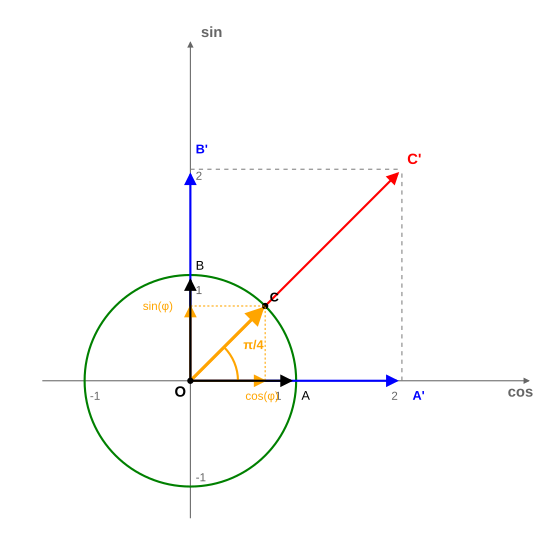
\includegraphics[width=0.9\textwidth]{./images/coordinates/linear_combination.png}

    \column{0.5\textwidth}
    \textbf{1.} Алгебраически: $\overrightarrow{OC'} = 2\cdot\overrightarrow{OB} + 2\cdot \overrightarrow{OA}$

    \vspace{0.3cm}

    \textbf{2.} Тригонометрически: $\overrightarrow{OC'} = r\cdot(\sin{\varphi}\cdot \overrightarrow{OB} + \cos{\varphi}\cdot\overrightarrow{OA})$, $r$ - во сколько раз нужно удлинить вектор $OC$ чтобы добраться до т.$C'$

    \vspace{0.3cm}

    \textbf{3.} Повернуть единичный вектор $\overrightarrow{OA}$ на угол $\varphi = \pi/4$ и домножить на $r$

    \vspace{0.3cm}

    \textbf{PS:} Можно заметить, что вектор $|\overrightarrow{OC}| = 1$ и работает теорема Пифагора $\cos^2{\varphi} + \sin^2{\varphi} = 1$
    \end{columns}

\end{frame}

% Слайд 13: Комплексная плоскость
\begin{frame}{Комплексная плоскость}
    \begin{columns}
        \column{0.5\textwidth}
        \begin{flushleft}
            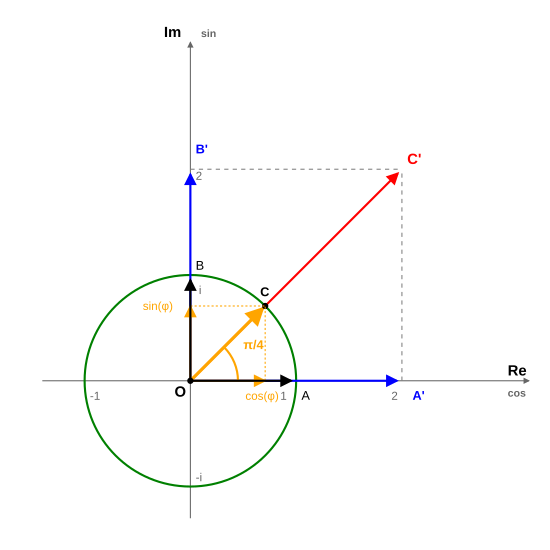
\includegraphics[width=0.9\textwidth]{./images/complex/complex_circle.png}
        \end{flushleft}
        \column{0.5\textwidth}
Пусть $\sqrt{-1} = i$, тогда $i^2=-1$.

Тогда например число $2+\sqrt{-121}$ можно представить так:
$2+\sqrt{-121} = 2 + 11\sqrt{-1} = 2 + 11i$

Помимо действительной оси $\mathbb{R}$ введем мнимую ось $\text{Im}$, на оси которой будут откладываться числа вида $a\cdot i = a\sqrt{-1}$ (например $i, -i, 2i, 11i, -2i, \frac{3}{4}i$ и т.д.), тогда точку $C'$, мы можем задать в виде $2+2i$
    \end{columns}
\end{frame}

% Слайд 14: Почему Im именно так
\begin{frame}{Комплексная плоскость}

Почему мы выбрали мнимую ось $\text{Im}$ именно таким образом.

Потому что умножение вектора на $-1$ означает поворот на $\pi$ (или на $180^\circ$), но $i^2 = -1$, что тоже означает поворот на $\pi$, а это значит, что умножение $i$ должено быть поворотом на $\frac{\pi}{2}$

Вектор $\overrightarrow{OA}\cdot i = \overrightarrow{OB}$

И для произвольного вектора $\overrightarrow{OC}$:

$\overrightarrow{OC}\cdot i = (\cos{\varphi} + i\cdot\sin{\varphi})\cdot i = i\cos{\varphi} + i^2\sin{\varphi} = -\sin{\varphi} + i\cos{\varphi}$

$\overrightarrow{OC}\cdot i = \cos{(\varphi+\frac{\pi}{2})} + i\cdot\sin{(\varphi+\frac{\pi}{2})}$

\end{frame}

% Слайд 15: Три формы записи
\begin{frame}{Три формы записи комплексных чисел}

    \begin{columns}
        \column{0.5\textwidth}
        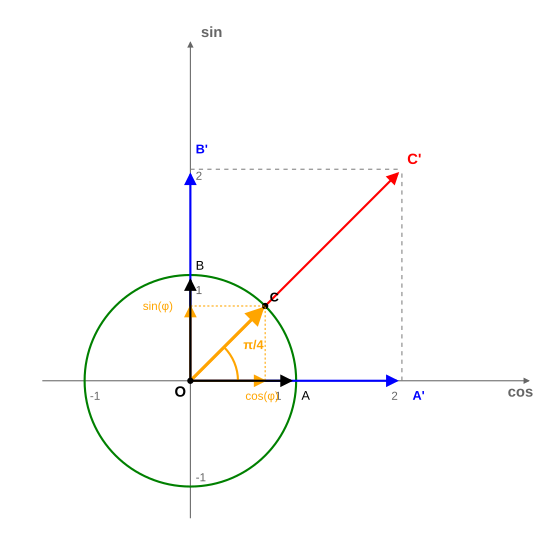
\includegraphics[width=0.9\textwidth]{./images/coordinates/linear_combination.png}

        \column{0.5\textwidth}
        \textbf{\textcolor{black}{У комплексного числа есть три формы записи:}}
        \begin{enumerate}
            \item \textbf{Алгебраическая}:

            $\overrightarrow{OC'} = 2\overrightarrow{OA} + 2\overrightarrow{OB} = 2\cdot \vec{1} + 2 \cdot \vec{i}$

            $C'=2+2i$

            \item \textbf{Тригонометрическая}:

            $\overrightarrow{OC'} = r\cdot(\cos{\varphi}\cdot\overrightarrow{OA} + \sin{\varphi}\cdot \overrightarrow{OB}) = r\cdot(\cos{\varphi}\cdot\vec{1} + \sin{\varphi}\cdot\vec{i})$

            $C' = r(\cos{\varphi} + i\cdot\sin{\varphi})$

            \item \textbf{Экспоненциальная}:

            $e^{i\varphi}=\cos{\varphi} + i\cdot\sin{\varphi}$ - формула Эйлера

            $C' = r\cdot e^{i\varphi}$
        \end{enumerate}
    \end{columns}

\end{frame}

% Слайд 16: Смысл формулы Эйлера
\begin{frame}{Смысл формулы Эйлера}

Формула Эйлера: $e^{i\varphi}=\cos{\varphi} + i\cdot\sin{\varphi}$

\vspace{0.3cm}

$(e^{i\varphi})' = i\cdot e^{i\varphi}$ \\
$(e^{i\varphi})'' = i^2\cdot e^{i\varphi} = -1\cdot e^{i\varphi}$ \\
$(e^{i\varphi})''' = -i\cdot e^{i\varphi}$ \\
$(e^{i\varphi})^{IV} = e^{i\varphi}$ \\
Заметим, что $(\cos{\varphi})^{IV} = \cos{\varphi}; \quad (\sin{\varphi})^{IV} = \sin{\varphi}$

Возведение $e^{i\varphi}$ означает поворот единичного вектора $\vec{1}$ на угол $\varphi$

\end{frame}

\begin{frame}{Смысл формулы Эйлера}

\begin{columns}[T]
\column{0.5\textwidth}
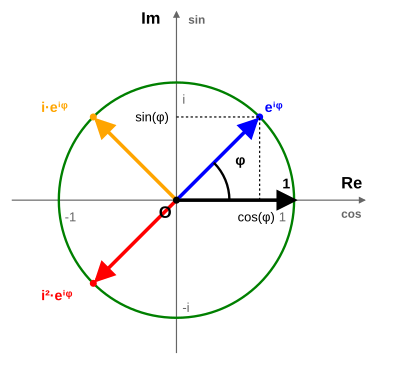
\includegraphics[width=0.6\textwidth]{./images/complex/derivative_of_exp.png}
\column{0.5\textwidth}
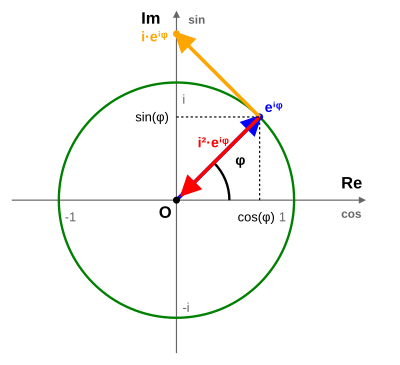
\includegraphics[width=0.6\textwidth]{./images/complex/derivative_of_exp2.png}
\end{columns}

Если геометрически $e^{i\varphi}$ это поворот на угол $\varphi$,

то в частности поворот вектора $\vec{1}$ на $\pi$ будет равен $-1$, т.е.
$$
\boxed{e^{i\pi} = -1}
$$
\end{frame}

% Слайд 17: Комплексная плоскость как область значений
\begin{frame}{Комплексная плоскость - область значений}

Комплексная плоскость - это не $x$, $y$ - оси, где $x$ - область определения, $y$ - область значений

В случае с функцией $e^{i\varphi}$, $\varphi$ - область определения, а комплексная плоскость - область значений.

\begin{columns}[T]
\column{0.5\textwidth}
\begin{figure}
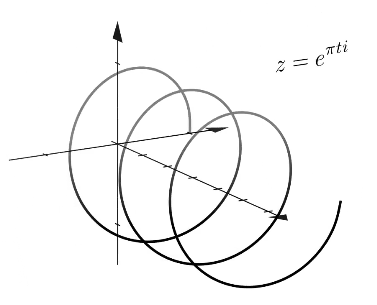
\includegraphics[width=0.3\textwidth]{./images/complex/spiral.png}
\caption{3D визуализация функции $e^{i\varphi}$}
\end{figure}
\column{0.5\textwidth}
\begin{figure}
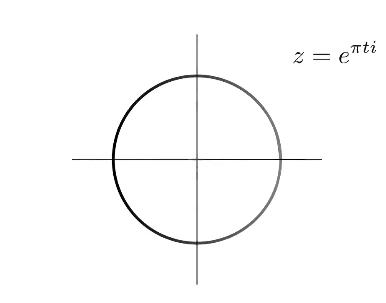
\includegraphics[width=0.3\textwidth]{./images/complex/Im_Re_projection.png}
\caption{Проекция функции $e^{i\varphi}$ на комплексную плоскость}
\end{figure}
\end{columns}

\begin{columns}[T]
\column{0.5\textwidth}
\begin{figure}
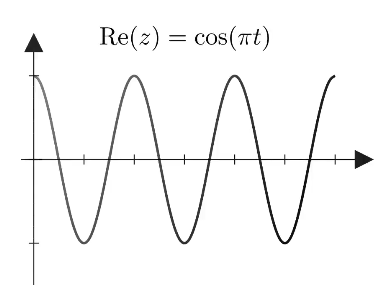
\includegraphics[width=0.3\textwidth]{./images/complex/Re_cos_projection.png}
\caption{Проекция функции $e^{i\varphi}$ на плоскость $\varphi$ Re}
\end{figure}
\column{0.5\textwidth}
\begin{figure}
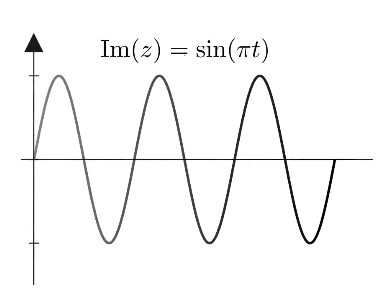
\includegraphics[width=0.3\textwidth]{./images/complex/Im_sin_projection.png}
\caption{Проекция функции $e^{i\varphi}$ на плоскость $\varphi$ Im}
\end{figure}
\end{columns}

\end{frame}

% Слайд 18: Сложение
\begin{frame}{Сложение комплексных чисел}
    \begin{columns}
        % Левая колонка для изображения
        \begin{column}{0.4\textwidth}
            \centering
            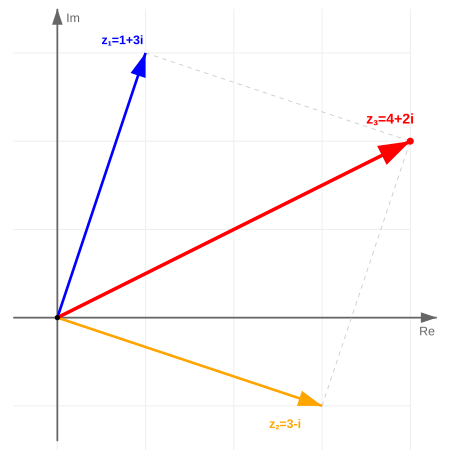
\includegraphics[width=\textwidth]{./images/complex/addition.png}
        \end{column}

        % Правая колонка для текста
        \begin{column}{0.6\textwidth}
            $z_1 = 1 + 3i,\; z_2 = 3 - i$ \\
            \vspace{0.5em}
            $z_3 = z_1 + z_2 = 1 + 3i + 3 - i$ \\
            \vspace{0.5em}
            $z_3 = 4 + 2i$
        \end{column}
    \end{columns}
    \end{frame}


% Слайд 19: Вычитание
\begin{frame}{Вычитание комплексных чисел}
    \begin{columns}
        % Левая колонка: изображение
        \begin{column}{0.5\textwidth}
            \centering
            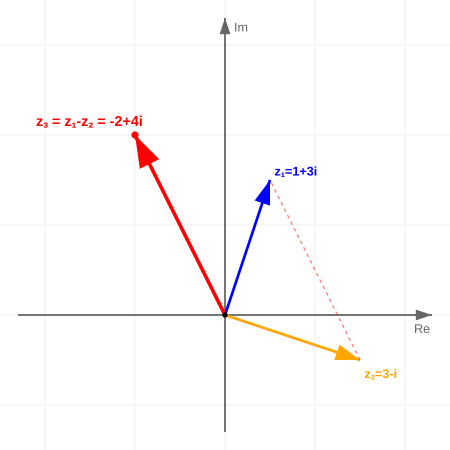
\includegraphics[width=0.9\textwidth]{./images/complex/substruction.png}
        \end{column}

        % Правая колонка: текст
        \begin{column}{0.5\textwidth}
            $z_1 = 1 + 3i,\; z_2 = 3 - i$ \\
            \vspace{0.5em}
            $z_3 = z_1 - z_2 = (1 - 3) + (3 - (-1))i$ \\
            \vspace{0.5em}
            $z_3 = -2 + 4i$
        \end{column}
    \end{columns}
\end{frame}


% Слайд 20: Умножение
\begin{frame}{Умножение комплексных чисел}
    \begin{columns}
        % Изображение слева
        \begin{column}{0.5\textwidth}
            \centering
            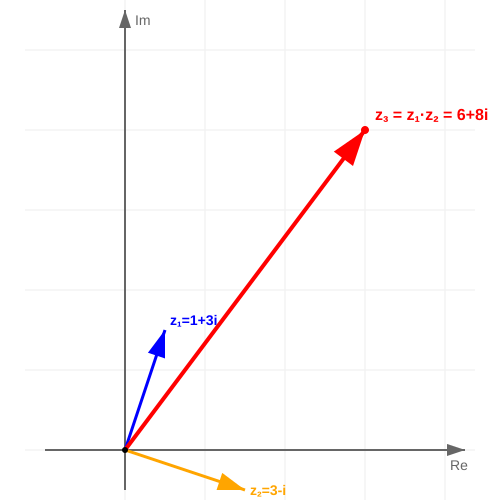
\includegraphics[width=0.9\textwidth]{./images/complex/multiplication.png}
        \end{column}

        % Текст справа
        \begin{column}{0.5\textwidth}
            $z_1 = 1 + 3i,\; z_2 = 3 - i$ \\
            \vspace{0.5em}
            $z_3 = z_1 \cdot z_2 = (1 + 3i)(3 - i)$ \\
            \vspace{0.5em}
            $z_3 = 3 - i + 9i - 3i^2$ \\
            \vspace{0.5em}
            $z_3 = 6 + 8i$
        \end{column}
    \end{columns}
\end{frame}


% Слайд 21: Деление
\begin{frame}{Деление комплексных чисел}
    \begin{columns}
        % Левая колонка для изображения
        \begin{column}{0.5\textwidth}
            \centering
            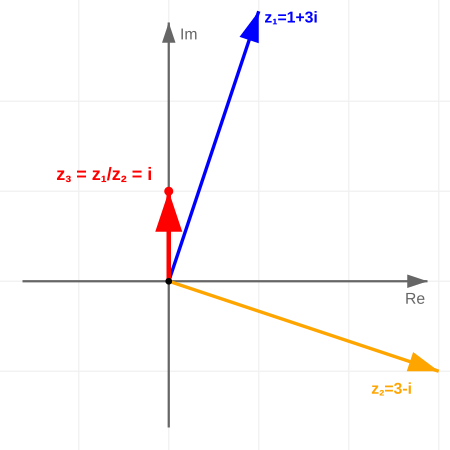
\includegraphics[width=0.9\textwidth]{./images/complex/division.png}
        \end{column}

        % Правая колонка для текста
        \begin{column}{0.5\textwidth}
            $$z_3 = \frac{1 + 3i}{3 - i} = \frac{(1 + 3i)(3 + i)}{(3 - i)(3 + i)} = $$
            $$z_3 = \frac{3 + i + 9i + 3i^2}{9 + 1} = \frac{10i}{10} = i$$
        \end{column}
    \end{columns}
\end{frame}


% Слайд 22: Корень из комплексного числа
\begin{frame}{Корень из комплексного числа}

\textbf{Основная идея:} у любого комплексного числа (кроме нуля) ровно $n$ корней $n$-й степени, и все они лежат на одной окружности.

Например из задачи Бомбелли:

$\sqrt[3]{2-11i}$

По формуле Муавра:
$$w_k = \sqrt[n]{r} \left( \cos \frac{\varphi + 2\pi k}{n} + i \sin \frac{\varphi + 2\pi k}{n} \right)$$
получим три корня:

$w_0 = 2 - i$ \\
$w_1 \approx -0.13 + 2.23i$ \\
$w_2 \approx -1.87 - 1.23i$

Один из которых $w_0$ был найден Бомбелли подбором.
Соответственно для $\sqrt[3]{2+11i}$ получим:

\begin{itemize}
    \item $w_0 = 2 + i$
    \item $w_1 \approx -1.87 + 1.23i$
    \item $w_2 \approx -0.13 - 2.23i$
\end{itemize}

$w_0 = 2 + i$ тоже был найден Бомбелли подбором.

\end{frame}

% Слайд 23: Задача
\begin{frame}{Задача}
\textbf{Задача:}
Выразить $\cos^7{x}$ через первые степени косинусов кратных аргументов.
\\(см. Андронов И.К, Окунев А.К. Курс тригонометрии, 1967г, стр. 622-623)

$\square$

Воспользуемся фактом, что:
$$
\left\{
\begin{matrix}
\cos{\varphi} = \frac{e^{i\varphi} + e^{-i\varphi}}{2} \\
\sin{\varphi} = \frac{e^{i\varphi} - e^{-i\varphi}}{2i}
\end{matrix}
\right .
$$

Это следует из формулы Эйлера $e^{i\varphi} = \cos{\varphi} + i\cdot\sin{\varphi}$:

$$
\left \{
\begin{matrix}
e^{i\varphi} = \cos{\varphi} + i\cdot\sin{\varphi} \\
e^{-i\varphi} = \cos{\varphi} - i\cdot\sin{\varphi}
\end{matrix}
\right .
$$

\end{frame}

% Слайд 24: Решение задачи
\begin{frame}{Задача - Решение}

А теперь применим формулу косинуса, выраженную через экспоненту и формулу бинома Ньютона:

$$
\cos^{7}x = \left( \frac{e^{ix} + e^{-ix}}{2} \right)^{7} = \frac{1}{2^{7}} (e^{ix} + e^{-ix})^{7} =
$$

$$
= \frac{1}{2^{7}} (e^{7xi} + 7e^{5xi} + 21e^{3xi} + 35e^{xi} + 35e^{-xi} + 21e^{-3xi} + 7e^{-5xi} + e^{-7xi}) =
$$

$$
= \frac{1}{2^{6}} \left( \frac{e^{7xi} + e^{-7xi}}{2} + 7 \frac{e^{5xi} + e^{-5xi}}{2} + 21 \frac{e^{3xi} + e^{-3xi}}{2} +  35 \frac{e^{xi} + e^{-xi}}{2} \right) =
$$

$$
= \frac{1}{2^{6}} (\cos 7x + 7 \cos 5x + 21 \cos 3x + 35 \cos x).
$$

$\blacksquare$

То же самое можно проделать для любых степеней $\sin^n{\varphi}$ или $\cos^n{\varphi}$ \\
\textbf{Применение:} если забыл на экзамене, как понижать степень у косинуса и синуса, то можно применить подобный подход

\end{frame}

\end{document}
